\subsection{Problema a resolver}
Este problema radica en una organización encargada de replicar contenido para su red de entrega de información en Internet. Para esto, dispone de $n$ servidores interconectados mediante $m$ enlaces $backbone$ de alta velocidad. El servidor $máster$ es el primero en recibir los nuevos datos a replicar y es el encargado de transmitir dicha información a otros servidores. Éstos guardarán su propia copia y la retransmitirán hasta que todos los servidores contengan la nueva información. Es importante considerar que todos los enlaces transmiten la misma información, que los $n$ servidores se encuentran interconectados por dichas conexiones y que los enlaces $backbone$ tienen costo en función del tráfico que transmiten.

La organización seleccionó dos consultoras con el fin de resolver los siguientes problemas:
\begin{itemize}
\item El primero se basa en hallar un algoritmo capaz de encontrar el camino mínimo entre un conjunto de servidores. En el contexto del problema, esto consiste en elegir los enlaces que permitan distribuir la información a todos los servidores con un costo mínimo.

\item El segundo consiste en encontrar el servidor $máster$ de forma tal que la replicación de la información, que empieza una vez que el $máster$ recibe la información y termina cuando todos los servidores tienen su copia, se realice en el mínimo tiempo posible. Para ello, se considera que la información tarda el mismo tiempo en atravesar cualquier enlace y que cada servidor transmite simultáneamente a todos los vecinos elegidos.
\end{itemize}
\textbf {Formatos de entrada y salida:}\newline
\newline
La entrada contiene varias instancias del problema. La primera línea de cada instancia contiene un entero positivo $n$ que indica la cantidad de servidores (numerados de 1 a $n$), un espacio, y un entero no negativo $m$ que corresponde a la cantidad de enlaces. A esta línea le siguen $m$ líneas con la descripción de cada enlace (números separados por un espacio):

$$a_{j}\ b_{j}\ ...\ c_{j}$$


donde \textbf{$a_{j}$} y \textbf{$b_{j}$} son los servidores que el enlace $j$ conecta y \textbf{$c_{j}$} es el costo de usar el enlace $j$ (entero no negativo). La entrada concluye con una línea comenzada por 0.\newline

La salida debe contener una línea por cada instancia de entrada, con el siguiente formato:

$$C\ U\ k\ e_{1}^1\ e_{2}^1\ e_{1}^2\ e_{2}^2\...\ e_{1}^k\ e_{2}^k$$


donde \textbf{$C$} es el costo total de la solución, $U$ es el servidor elegido como $máster$, $k$ es la cantidad de enlaces y $e_{1}^i$ y $e_{2}^i$ son los extremos del $i$-ésimo enlace de la solución obtenida, para $i\ \in$ [1,$k$].\newline

En lo que sigue, presentaremos dos ejemplos del problema a resolver:
\begin{itemize}
\item {\large{\textbf{Ejemplo 1:}}}\newline
\newline
El siguiente ejemplo consiste en un caso simple de la situación a resolver con la particularidad de que existe más de una solución posible al problema. Como puede observarse, tanto el enlace (1,5) como el (5,4) forman parte de la solución óptima, pero de éstos se elige únicamente uno.\newline
\newline
\textbf{Formato de entrada:}
$$5\ 6$$
$$1\ \ 2\ \ 2$$
$$1\ \ 3\ \ 1$$
$$1\ \ 5\ \ 2$$
$$2\ \ 3\ \ 1$$
$$3\ \ 4\ \ 1$$
$$4\ \ 5\ \ 2$$

\begin{figure}[H] %[h] Aqui [b] para button [t] para top
\begin{center}
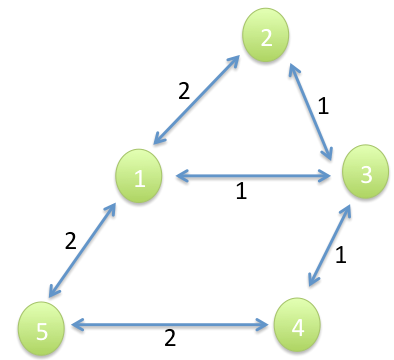
\includegraphics[width=210pt]{../imgs/ejemplo1ej2ent.jpg}
\caption{Ejemplo 1 - entrada.}
\end{center}
\end{figure}

\textbf{Formato de salida:}
$$5\ \ 2\ \ 4\ \ 1\ \ 2\ \ 1\ \ 5\ \ 2\ \ 3\ \ 3\ \ 4$$

\begin{figure}[H] %[h] Aqui [b] para button [t] para top
\begin{center}
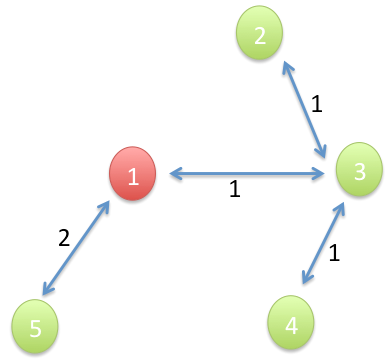
\includegraphics[width=210pt]{../imgs/ejemplo1ej2sal.jpg}
\caption{Ejemplo 1 - salida.}
\end{center}
\end{figure}
\item {\large{\textbf{Ejemplo 2:}}}\newline
\newline
Este ejemplo consiste en un caso usual de la situación planteada en el que puede verse de forma simple y clara la elección que debe realizar el algoritmo para hallar la solución óptima.\newline
\newline
\textbf{Formato de entrada:}
$$5\ 6$$
$$1\ \ 2\ \ 2$$
$$1\ \ 3\ \ 3$$
$$2\ \ 3\ \ 1$$
$$3\ \ 4\ \ 2$$
$$3\ \ 5\ \ 2$$
$$4\ \ 5\ \ 1$$

\begin{figure}[H] %[h] Aqui [b] para button [t] para top
\begin{center}
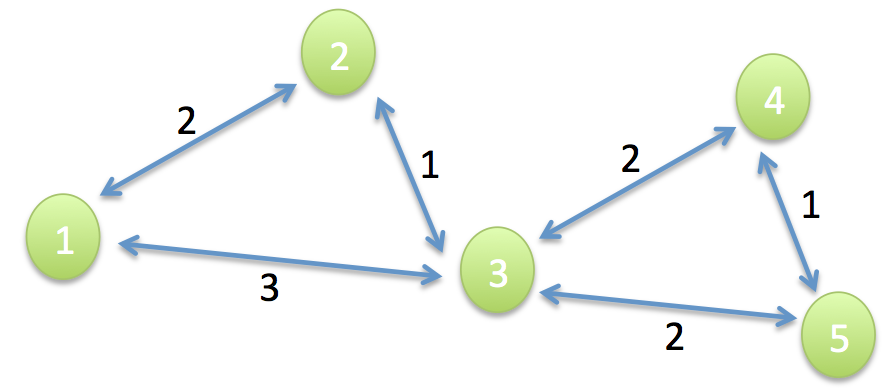
\includegraphics[width=300pt]{../imgs/ejemplo2ej2ent.jpg}
\caption{Ejemplo 2 - entrada.}
\end{center}
\end{figure}

\textbf{Formato de salida:}
$$8\ \ 3\ \ 4\ \ 1\ \ 3\ \ 2\ \ 3\ \ 3\ \ 4\ \ 3\ \ 5$$

\begin{figure}[H] %[h] Aqui [b] para button [t] para top
\begin{center}
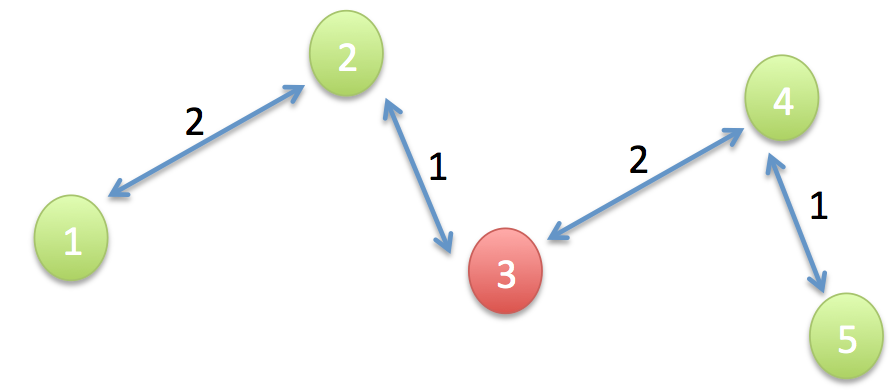
\includegraphics[width=300pt]{../imgs/ejemplo2ej2sal.jpg}
\caption{Ejemplo 2 - salida.}
\end{center}
\end{figure}

\subsection{Minimización de enlaces}
\subsubsection{Resolución coloquial}

 El problema planteado consiste en conectar todos los servidores de la red de forma tal que el costo de transmisión de datos sea el mínimo. Para poder resolver esto, decidimos utilizar un algoritmo que encontrara un Árbol Generador Mínimo\footnote{El peso de un árbol generador es la suma de los pesos de las aristas del árbol. Un árbol generador mínimo es uno con peso mínimo.} que contuviera los enlaces de menor peso necesarios para unir a todos los servidores. Para ello, utilizamos el algoritmo de $Kruskal$. Éste genera un conjunto de árboles que representan los nodos del grafo original. El algoritmo toma la menor arista (según su peso) y evalúa si sus extremos pertenecen a árboles distintos. En caso de así serlo, los une y agrega la arista al árbol generador mínimo. Si, por el contrario, los extremos forman parte del mismo árbol, el algoritmo descarta dicha arista.\newline
\newline
El pseudocódigo del algoritmo mencionado es el siguiente: \newline
\newline

\begin{algorithm}[H]
	\SetAlgoLined
	\caption{kruskal}
	\KwIn{Entero $CantidadServidores$, Grafo $G$}
	\KwOut{Grafo $Gr$}
    
    $//G = (V,E)$ \\
    ordenarDeMenorAMayorPorPeso $E$\\  
    \\ 
    Grafo $Gr \leftarrow$ $<>$\\
	\ForAll{$E$}{
        Entero $nodoA \leftarrow$ PrimerVertice $E$\\
        Entero $nodoB \leftarrow$ SegundoVertice $E$\\
        \If{find(nodoA) != find(nodoB)}{\\
            union(find($nodoA$), find($nodoB$)) \\
            Marcar($E$)
        }
	}\\
    \ForAll{$E$}{
        \If{EstaMarcado?($E$)}{\\
            Insertar($Gr$,$E$)   \\
        }
	}

	\textbf{devolver} $Gr$
\end{algorithm}

\newline
Para lograr que el algoritmo de Kruskal fuera más eficiente, decidimos aplicarle una mejora tanto a la función union como a la función find.\newline
\newline
En el caso de la función $find$, decidimos aplicar el método de $compresión\ de\ caminos$ que, al momento de retornar la raíz en la recursión, actualiza el padre de cada vértice visitado. Luego, cada nodo ya visitado tiene como padre a la raíz.\newline
\newline
Para la función $union$, implementamos el método $unión\ por\ rango$. Éste une el árbol de menor rango con la raíz del de mayor rango. Luego, la altura resultante es igual a la mayor de los dos. Si no se aplicara dicha función, la altura resultante sería la del árbol más grande +1 dado que éste se colocaría como hijo de la raíz del de menor tamaño. \newline
\newline
Los pseudocódigos de dichos algoritmos son los que se presentan a continuación:\newline
\newline
\begin{algorithm}[H]
	\SetAlgoLined
	\caption{find}
	\KwIn{Entero $nodo$, vector$<$Entero$>$ $padre$}
	\KwOut{Entero res}
	\If{nodo = Raiz(nodo)}{\textbf{devolver} $nodo$}
    
	\textbf{devolver} $Raiz(nodo) \leftarrow$ find(Raiz($nodo)$)
\end{algorithm}

\begin{algorithm}[H]
	\SetAlgoLined
	\caption{union}
	\KwIn{Entero $nodoA$, Entero $nodoB$, vector$<$Entero$>$ $padre$}
	\KwOut{Entero res}
	\eIf{AlturaDeLaComponente $nodoA$ $>$ AlturaDeLaComponente $nodoB$}{Raiz($nodoB$) = $nodoA$}{
    Raiz($nodoA$) = $nodoB$\\
    AlturaDeLaComponente $nodoB$++}
\end{algorithm}

Donde la función $Raiz(x)$ devuelve la raíz del árbol conteniendo el nodo $x$ y la función $AlturaDeLaComponente(x)$ devuelve la altura del árbol que comprende a $x$.

\subsubsection{Demostración de correctitud}

Para demostrar la correctitud de nuestro algoritmo, debemos probar que se cumplen las siguientes propiedades:
\begin{itemize}
\item Se unen todos los servidores mediante enlaces $backbone$.
\item La solución es óptima, es decir, no existe otra combinación de enlaces que una a todos los servidores y cuyo costo sea menor.
\end{itemize}

\newline

\textbf{Se unen todos los servidores mediante enlaces backbone:} \newline
\newline
La entrada de nuestro algoritmo es un grafo conexo. Esto significa que, para cualquier par de vértices ($v_{1}$, $v_{2}$) del grafo, existe al menos un camino que los une. \newline  
\newline
Sea $G$ el grafo de entrada de $n$ nodos y $m$ aristas, y $G'$ uno conformado por $n$ componentes conexas, donde cada una de ellas es un vértice de $G$.
En primer lugar, nuestro algoritmo comprueba si la inserción de cada arista de $G$ en $G'$ genera algún ciclo. En caso de producirlo, no la agrega, caso contrario sí. En otras palabras, se insertan en $G'$ las aristas que únicamente unen dos componentes conexas distintas. Al repetir dicho procedimiento para las $m$ aristas de $G$, obtenemos un grafo sin ciclos que une a los $n$ nodos. Esto es posible dado que $G$ es conexo.
\newline
\newline
\textbf{La solución es óptima:} \newline
\newline
Sea $G$ un grafo conexo, $E$ un arreglo de aristas de $G$ ordenadas por peso y $G'$ un bosque con $n$ árboles, que representan a los nodos de $G$. 
Probemos que si $G$ es conexo y $G'_{k}$ tiene $i$ árboles mínimos $\Rightarrow\ G'_{k+1}$ tiene $i$ o $i-1$ árboles mínimos.\newline

 Sea $e_{k}$ la $k$-ésima arista perteneciente a $E$ y sean $v_{1}$ y $v_{2}$ sus extremos. Si $v_{1}$ y $v_{2}$ pertenecen al mismo árbol, no agregamos $e_{k}$ para no generar un ciclo y quitarle la propiedad de árbol. Entonces, $G'_{k+1}$ queda conformado por $i$ árboles mínimos.\newline
 \newline
Por otro lado, si $v_{1}$ y $v_{2}$ no pertenecen al mismo árbol, $e_{k}$ es la arista de menor peso que los une. Esto se debe a que las $k-1$ aristas anteriores ya conforman $G'_{k}$ o no, de acuerdo a si la inserción de las mismas generan ciclos. Al agregar $e_{k}$ en $G'_{k}$, se forma un nuevo árbol de peso mínimo por estar conformado por dos árboles mínimos y la arista de menor peso entre todas las que los conectan. Por lo tanto, $G'_{k+1}$ queda conformado por $i-1$ árboles mínimos.\newline \newline
Al ejecutar este proceso $m$ veces, en $G'$ se obtiene una única componente conexa con $n-1$ aristas (no pueden ser más dado que sino $G'$ no sería un árbol).

\subsubsection{Complejidad del algoritmo}

  Sea $n$ la cantidad de servidores que posee una red de entrega de contenidos (nodos) y $m$ la cantidad de enlaces que los unen (aristas). Supongamos que tenemos un grafo completo, entonces $m$ = $\frac{n(n-1)}{2}$. Luego, $m \leq \frac{n(n-1)}{2} \leq n^{2}$. 
 
  Para analizar la complejidad de nuestro algoritmo, veámoslo por partes: 
  
 \begin{itemize}
	
 \item Algoritmo de $Kruskal$
 
 La función $ordenarDeMenorAMayorPorPeso$ se encuentra implementada con la función $sort$\footnote{http://en.cppreference.com/w/cpp/algorithm/sort}. La misma se aplica sobre un vector que contiene todas las aristas ingresadas por parámetro. Como dicho vector tiene tamaño $m$, la complejidad de aplicar esta función resulta $\mathcal{O}(m\ log\ m)$. Al acotar $m$ por $n^{2}$, obtenemos, como complejidad final, $\mathcal{O}(n^{2}\ log\ n^{2})$.\newline

 Luego, se ingresa en el ciclo principal que recorre todas las aristas del grafo en $\mathcal{O}(m)$ = $\mathcal{O}(n^{2})$. En él, se calculan las funciones $PrimerVertice$ y $SegundoVertice$ con una complejidad de $\mathcal{O}(1)$ ya que dicha información se encuentra alojada en la estructura. Posteriormente, se calcula $find$ a cada uno de los nodos cuya complejidad es O($ACK(n)$) amortizado, donde $ACK$ corresponde a la función de Ackermann acotada por $\mathcal{O}(1)$ amortizado\footnote{TARJAN, ROBERT ENDRE (1975). "Efficiency of a Good But Not Linear Set Union Algorithm". Journal of the ACM 22}.\newline

 Luego, se controla si los nodos pertenecen o no a la misma componente conexa. En caso de que no pertenezcan, se aplican las funciones $union$ y $Marcar$. La función $union$, al igual que $find$, está acotada por la función de Ackermann, o sea que por $\mathcal{O}(1)$ amortizado. Por otro lado, $Marcar$ indica que la arista que se le pasa por párametro debe ser insertada posteriormente en un grafo. Esta acción se realiza en $\mathcal{O}(1)$ ya que se utiliza un arreglo al cual se accede de forma directa.\newline
 
 Por lo tanto, podemos concluir que las ejecuciones dentro del ciclo tienen una complejidad temporal de $\mathcal{O}(1)$. Luego, la complejidad del ciclo es de $\mathcal{O}(n^{2})$. \newline

 Por último, se recorren todas las aristas para ver si fueron marcadas o no. Si lo fueron, se las inserta en un grafo. Este grafo esta implementado sobre un vector al cual se le redefine su tamaño mediante la funcion $resize$\footnote{http://www.cplusplus.com/reference/vector/vector/resize/} con una complejidad de $\mathcal{O}(n-1)$. Dicha inserción se realiza mediante la función $Insertar$ que agrega la arista en $\mathcal{O}(1)$. Por lo tanto, el costo de este ciclo es $\mathcal{O}(n-1)$.
\newline
\newline
 Finalmente, al sumar las complejidades de $ordenarDeMenorAMayorPorPeso$ con la del ciclo principal, obtenemos que la complejidad temporal del Algoritmo de $Kruskal$ está dada por $\mathcal{O}(n^{2}\ log\ n^{2})$ + $\mathcal{O}(n^{2})$, siendo estrictamente menor que $\mathcal{O}(n^{3})$.\newline
 
 \item Cálculo del costo de la red

  Para poder calcular el costo temporal de la red, debe considerarse que se recorren todas las aristas devueltas por el algoritmo de $Kruskal$ y se suman sus respectivos pesos. Dado que dicho algoritmo devuelve un árbol, la cantidad de aristas equivale a $n - 1$, por lo tanto la complejidad del Cálculo del costo de la red es $\mathcal{O}(n)$.\newline
  
	\item Generación de la lista de adyacencia
 
  Para poder generar la lista de adyacencia, creamos un vector de vectores. El vector principal es de $n$ elementos y en cada posición se guarda un vector conteniendo los nodos adyacentes. Para poder rellenarlo, se recorre el vector de aristas resultante de aplicar $Kruskal$ ($\mathcal{O}(n)$) y se obtienen los extremos de cada arista en $\mathcal{O}(1)$. Luego, se inserta el primer nodo en la lista del segundo y el segundo en la lista del primero para cada par de aristas. Dicha inserción se realiza con $push\_back()$ ($\mathcal{O}(1)$)\footnote{http://www.cplusplus.com/reference/vector/vector/push_back/}. Por lo tanto, generar la lista de adyacencia tiene una complejidad de $\mathcal{O}(m)^*\mathcal{O}(1)$ y, al acotar $m$ por $n^{2}$, ésta resulta $\mathcal{O}(n^{2})$.
	
\end{itemize}

 Finalmente, la complejidad final del algoritmo resulta de sumar las fracciones mencionadas anteriormente. Luego, ésta es $\mathcal{O}(n^{2}\ log\ n^{2})$ + $\mathcal{O}(n)$ + $\mathcal{O}(n^{2})$ que es estrictamente menor a $\mathcal{O}(n^{3})$.

\subsection{Selección de servidor $máster$}

\subsubsection{Resolución coloquial}
El problema a resolver consiste en encontrar el nodo del grafo generado en el ítem $a)$ desde el que la replicación de contenido se realice en la menor cantidad de pasos posibles. Para esto, decidimos utilizar un algoritmo que nos devolviera el camino más largo del árbol a procesar. A partir de éste, se devuelve el nodo del centro que es el que menos pasos debe realizar para llegar a los más alejados del árbol.\newline
\newline
El algoritmo que utilizamos para encontrar el camino de longitud máxima es $BFS$ (Búsqueda en anchura). Éste toma un nodo inicial y devuelve el más distante a él. Para ello, procede recorriendo desde el nodo inicial y explorando todos sus nodos adyacentes de manera sucesiva hasta recorrer todo el árbol. La particularidad del algoritmo es que recorre el árbol por niveles, luego, el último nodo que visita pertenece al último nivel del árbol, resultando éste el más alejado del inicial.\newline
\newline
Como $BFS$ retorna el camino más largo desde un nodo inicial, decidimos aplicarlo dos veces sobre nuestro grafo. La primera vez lo hicimos sobre el $nodo 1$, cuya existencia está asegurada para cualquier grafo no nulo. De este modo, obtenemos el nodo más distante a éste, que es a su vez utilizado para ejecutar el algoritmo por segunda vez. De esta forma, obtenemos el camino de longitud máxima conformado por el nodo resultante de la primera pasada de $BFS$ y el de la segunda.\newline
\newline
El pseudocódigo del algoritmo $BFS$ es el siguiente:\newline
\newline
\begin{algorithm}[H]
	\SetAlgoLined
	\caption{BFS}
	\KwIn{Entero $nodoInicial$, Entero $CantidadNodos$, Grafo $G$}
	\KwOut{Par$<$Entero, Entero$>$ $res$}
	
    encolar($Q$, $nodoInicial$)\\
    marco $nodoInicial$\\
    Distancia($nodoInicial$) \leftarrow 0\\
    \While{!vacia(Q)}{
        $nodo \leftarrow$ extraer($Q$)\\
         
	    \ForAll{$v \in$ Adyacentes($nodo$)}{
            \If{$v$ no esta marcado}{\\
                marco $v$ \\
                Distancia($v$) \leftarrow Distancia($nodo$) +1\\
                encolar($Q$, $v$)   \\
            }
        }
	}
    
    $primero(res) \leftarrow$ $nodo$\\
    $segundo(res) \leftarrow$ nodoDelMedio\\
    
	\textbf{devolver} $res$
\end{algorithm}

Donde $marco$ evalúa si ese nodo ya fue visitado, $Distancia$ indica la distancia de ese nodo al $nodoInicial$, $Adyacentes$ devuelve una lista con todos sus nodos adyacentes y $nodoDelMedio$ retorna el nodo que se encuentra en la mitad del camino generado entre el nodo inicial y el que devuelve el $BFS$.

\subsubsection{Demostración de correctitud}
Demostremos que nuestro algoritmo encuentra, efectivamente, el nodo central del camino más largo de un árbol. Para lograr esto, se realiza $BFS$ una vez para obtener uno de los extremos de este camino. Posteriormente, se repite la ejecución con ese extremo para obtener el camino más largo.\newline
Para demostrar esto, necesitamos probar dos cosas: 
\begin {itemize}
\item La primera ejecución de $BFS$ nos devuelve uno de los extremos del camino más largo del árbol.
\item La segunda ejecución nos devuelve el camino más largo del árbol.
\end{itemize}
\newline
\textbf{La primera ejecución de $BFS$ nos devuelve un extremo del camino más largo del árbol:} \newline

Sea $G$ un árbol y $v_{1}$, $v_{2}$ dos de sus vértices. Sabemos que existe un camino entre $v_{1}$ y $v_{2}$ que los une.

 Por otro lado, el algoritmo $BFS$\footnote{Cormen, Thomás H., Charles E. Leiserson, and Ronald L. Rivest. Chapter 22.2} toma el nodo inicial de un árbol y devuelve el más distante a él, junto con el camino máximo entre estos.\newline

Demostremos por el absurdo que, dado cualquier nodo del árbol, $BFS$ retorna uno de los extremos del camino máximo. Para ello, miremos todos los casos en los que esto no ocurre y probemos que ninguno de éstos es posible.\newline
\begin {itemize}
\item El nodo final no es una hoja de $G$. \newline
Sea $v_{1}$ el nodo inicial y $v_{2}$ el nodo final del algoritmo $BFS$. Si $v_{2}$ no es una hoja, existe un nodo $v'$ que sí lo es (pues es un árbol y no posee ciclos) y un camino $c$ que une a los nodos $v'$ y $v_{2}$. Entonces, $v_{2}$ no es el nodo más distante a $v_{1}$ ya que el camino que une $v_{1}$ con $v'$ es más largo que el que une $v_{1}$ con $v_{2}$. Pero esto contradice la hipótesis de la que partimos. Luego, es absurdo.\newline  
\item El nodo inicial pertenece al camino máximo del árbol y el final no.

\begin{figure}[H] %[h] Aqui [b] para button [t] para top
%\begin{center}
\begin{minipage}[H]{260pt}
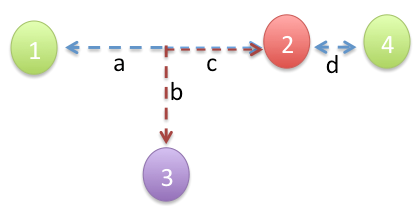
\includegraphics[width=260pt]{../imgs/ej2casos02.jpg}
%\end{center}
\end{minipage}
\hfill
  \fbox{\begin{minipage}[H]{150pt}
    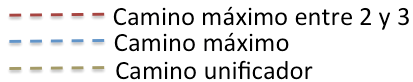
\includegraphics[width=150pt]{../imgs/leyendacasosej2.jpg}
  \end{minipage}}
\caption{Segundo caso posible.}
\end{figure}

A partir del gráfico anterior, supongamos que el camino rojo representa al máximo que resulta del algoritmo $BFS$ luego de haberlo aplicado sobre el nodo 2. \newline
Por otro lado, supongamos que dicho algoritmo retorna al nodo 3 como el más lejano del 2. Como el nodo 3 se encuentra más lejos del 2 que el 1, $b \geq a$. 
\begin{itemize}
\item $a$ = $b$: En este caso, ambos caminos hubieran sido correctos ya que dist(4,1) sería igual a dist(4,3). 
\item $a<b$: Si este caso sucediera, $b$ debería formar parte del camino máximo del árbol. Esto se debe a que el camino más largo del árbol debe estar conformado por los caminos $c$-$d$ y el máximo entre $a$ y $b$. Por lo tanto, si $b>a$, el camino azul no sería el máximo. Luego, es absurdo suponer que el extremo del camino máximo retornado por $BFS$ no pertencía al camino máximo del árbol.\newline
\end{itemize}
\item Tanto el nodo inicial como el final no pertenecen al camino máximo del árbol. \newline \newline
Sea el camino $azul$ el máximo del árbol cuyos extremos son los nodos 1 y 4. Supongamos que el camino $rojo$ representa al camino devuelto por $BFS$ al aplicarlo sobre el nodo 2. En este caso, tenemos dos opciones posibles: El camino $azul$ comparte un tramo con el camino $rojo$ o no comparte ninguno. Veamos cada una de ellas por separado. \newline
\begin{itemize}
\item El camino azul comparte un tramo con el camino rojo. \newline
\begin{figure}[H] %[h] Aqui [b] para button [t] para top
%\begin{center}
\begin{minipage}[H]{240pt}
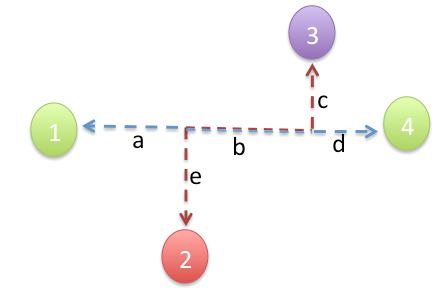
\includegraphics[width=240pt]{../imgs/ej2casos01.jpg}
\end{minipage}
\hfill
  \fbox{\begin{minipage}[H]{150pt}
    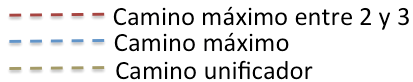
\includegraphics[width=150pt]{../imgs/leyendacasosej2.jpg}
  \end{minipage}}
\caption{Tercer caso posible.}
%\end{center}
\end{figure}
Supongamos que el algoritmo $BFS$ devuelve el nodo 3 como el más alejado al 2. Entonces, podemos deducir que:
\begin {itemize}
\item $c$ = $d$: Ambas soluciones son correctas.
\item $c > d$: Si este caso ocurriera, $c$ debería formar parte del camino máximo del árbol. Luego, el camino azul no sería el máximo. Por lo tanto, resulta absurdo suponer que el extremo del camino máximo otorgado por $BFS$ no pertencía al camino máximo del árbol. \newline
\end{itemize}
\item El camino azul no comparte nigún tramo con el rojo.
\begin{figure}[H] %[h] Aqui [b] para button [t] para top
%\begin{center}
\begin{minipage}[H]{240pt}
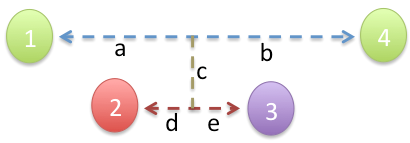
\includegraphics[width=240pt]{../imgs/ej2casos03.jpg}
\end{minipage}
\hfill
  \fbox{\begin{minipage}[H]{150pt}
    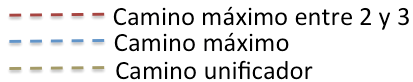
\includegraphics[width=150pt]{../imgs/leyendacasosej2.jpg}
  \end{minipage}}
\caption{Cuarto caso posible.}
%\end{center}
\end{figure}
\end{itemize}
\end{itemize}

Supongamos que el algoritmo $BFS$ nos devuelve el nodo 3 como el más alejado del 2. Entonces, podemos deducir que:
\begin {itemize}
\item $(a \cup c)$ = $e$: Ambas soluciones son correctas.
\item $(b \cup c)$ = $e$: Ambas soluciones son correctas.
\item $(a \cup c) < e$: Si este caso sucediera, $e \cup c$ debería formar parte del camino máximo del árbol. Pero entonces el camino azul no sería el máximo, lo que resulta absurdo.
\item $(b \cup c) < e$: En este caso, $e \cup c$ debería formar parte del camino máximo del árbol. Luego, resulta absurdo.
\newline
\end{itemize}
\end{itemize}

Luego, logramos demostrar que la primera ejecución de $BFS$ retorna como resultado una hoja del árbol al que se le aplica. Además, probamos que dicha hoja pertenece obligatoriamente al camino máximo. Por lo tanto, podemos concluir que la primera ejecución devuelve uno de los dos extremos del camino más largo del árbol. \newline
\newline
\textbf{La segunda ejecución nos devuelve el camino más largo del árbol.} \newline

A la segunda ejecución del algoritmo le ingresa por párametro uno de los extremos del camino más largo del árbol. Luego de dicha ejecución, se obtiene entonces el otro extremo. Una vez encontrado el camino más largo, éste debe ser recorrido hasta hallar el nodo intermedio.
\subsubsection{Complejidad del algoritmo}

Sea $n$ la cantidad de servidores que posee una red de entrega de contenidos (nodos) y $m$ la cantidad de enlaces que los unen (aristas). Dado que procesamos un árbol, sabemos que $m$ = $n-1$, en particular, $m \leq n$.\newline

Para analizar la complejidad de nuestro algoritmo, vamos a calcular la complejidad del algoritmo $BFS$.
\newline

Lo primero que hace $BFS$ es crear dos arreglos de tamaño $n$, uno para almacenar las distancias y el otro para ir marcando los nodos por los cuales ya ocurrió. Crear ambos arreglos tiene una complejidad de $\mathcal{O}(n)$. Además se encola, mediante la función $push$\footnote{http://www.cplusplus.com/reference/queue/queue/push/}, el primer elemento. La complejidad de esta función es $\mathcal{O}(1)$ ya que la estructura interna de la cola está implementada sobre $double-ended\ queue$ y su función $push\_back$ tiene complejidad $\mathcal{O}(1)$.
\newline

Posteriormente, se ingresa a un ciclo que se ejecuta mientras la cola no se encuentre vacía. Esto se controla utilizando la función $empty$\footnote{http://www.cplusplus.com/reference/queue/queue/empty/} cuya complejidad es de $\mathcal{O}(1)$.
\newline

Una vez dentro del ciclo, se aplica la función $front$\footnote{http://www.cplusplus.com/reference/queue/queue/front/} sobre la cola para poder obtener el valor del primer nodo. Luego se usa la función $pop$\footnote{http://www.cplusplus.com/reference/queue/queue/pop/} para quitar este valor de la cola. Ambas funciones tienen una complejidad constante. \newline

Por ultimo, se ejecuta un ciclo el cual recorre un vector de nodos adyacentes. Para cada uno de estos nodos, el algoritmo se fija si fue marcado o no. En caso afirmativo, aplica inserciones sobre arreglos con un $push$; Por lo tanto, dentro del ciclo la complejidad es constante.

Como podemos observar, el ciclo principal se ejecuta $n$ veces ya que todos los nodos son colocados una sola vez en la cola. Además, dentro de este se encuentra otro bucle el cual recorre todos los nodos adyacentes a cada vértice. Es por esto que en el ciclo principal se terminan recorriendo $m$ aristas en las $n$ iteraciones . Por lo tanto la complejidad del ciclo principal es de $\mathcal{O}(n)$ + $\mathcal{O}(m)$ que es igual a $\mathcal{O}(n)$.
\newline

En resumen, el ciclo principal tiene complejidad $\mathcal{O}(n)$ y las funciones que se encuentran antes que este, tienen complejidad $\mathcal{O}(n)$ por lo tanto, la complejidad del algoritmo es $\mathcal{O}(n)$

\subsubsection{Instancias posibles}

Para verificar la correctitud de nuestro programa, dispusimos variar estratégicamente las instancias de entrada al ejecutarlo.
\begin{itemize}
\item En primer lugar, ejecutamos el programa ingresando un caso con una única arista. De este modo, logramos corroborar el correcto funcionamiento de nuestro algoritmo para este tipo de casos borde.\newline
\textbf{Parámetro de entrada:} $$2\ \ 1 $$
$$1\ \ 2\ \ 13 $$
\textbf{Parámetro de salida:} $$13\ \ 2\ \ 1\ \ 1\ \ 2$$

\item Posteriormente, ejecutamos el programa ingresando un solo nodo. De esta forma, pudimos controlar que ocurría si no se ingresaban aristas.\newline
\textbf{Parámetro de entrada:} $$1\ \ 0 $$
\textbf{Parámetro de salida:} $$0\ \ 1\ \ 0$$

\item Por otra parte, quisimos ver un caso que minimizara los costos en el primer ítem pero que ralentizara, luego, el trabajo del $máster$. Este caso nos permite ver que no siempre es mejor elegir el camino mínimo antes que el $máster$, sino que depende lo que se priorice (en este caso el costo final).\newline
\textbf{Parámetro de entrada:} $$5\ \ 5$$
$$1\ \ 3\ \ 10$$
$$3\ \ 2\ \ 10$$
$$3\ \  4\ \  10$$
$$3\ \  5\ \  10$$
$$4\ \  5\ \  5$$
\textbf{Parámetro de salida:} $$35\ \ 3\ \ 4\ \ 4\ \ 5\ \ 1\ \ 3\ \ 3\ \ 2\ \ 3\ \ 4 $$

\item También, buscamos una situación inversa al caso anterior, es decir, en el que la elección de conexiones con menor costo permitiera, luego, encontrar un $máster$ eficiente.\newline
\textbf{Parámetro de entrada:} $$5\ \  6$$
$$1\ \  2\ \  12$$
$$1\ \  3\ \ 14$$
$$1\ \  4\ \  10$$
$$2\ \  4\ \ 9$$
$$3\ \  4\ \  10$$
$$4\ \  5\ \ 11$$
\textbf{Parámetro de salida:} $$40\ \ 4\ \ 4\ \ 2\ \ 4\ \ 1\ \ 4\ \ 3\ \ 4\ \ 4\ \ 5$$

\item Para finalizar, buscamos un caso que tuviera varias soluciones óptimas en el primer ítem pero que, cada una de estas, implique un costo de replicación de datos distintos (segundo ítem).\newline
\textbf{Parámetro de entrada:} $$5\ \ 8$$
$$1\ \ 2\ \ 1$$
$$2\ \ 3\ \ 1$$
$$3\ \ 4\ \ 1$$
$$4\ \ 1\ \ 1$$
$$5\ \ 1\ \ 1$$
$$5\ \ 2\ \ 1$$
$$5\ \ 3\ \ 1$$
$$5\ \ 4\ \ 1$$
\textbf{Parámetro de salida:} $$4\ \ 2\ \ 4\ \ 1\ \ 2\ \ 2\ \ 3\ \ 3\ \ 4\ \ 5\ \ 1$$

\end{itemize}

De este modo, logramos abarcar los casos límite en los que la implementación pudiera haber encontrado algún problema. Dado que los resultados obtenidos fueron los esperados, determinamos que para todas las instancias válidas posibles de entrada nuestra implementación resulta correcta.

\subsubsection{Experimentación}

Para las pruebas de complejidad empírica, generamos instancias aleatorias de costos de los enlaces y servidores variando la cantidad de los mismás. Estas instancias fueron generadas en $C++$ con la función $rand()$ que recibe como parametro una semilla generada por bash. La cantidad de trabajos generados se comprendió entre 200 y 46800, agregando de a 200 en cada iteración. Las mediciones de tiempo en microsegundos se realizaron con la función $high\ resolution\ clock$\footnote{http://en.cppreference.com/w/cpp/chrono/high\_resolution\_clock} de la librería $Chrono$ de $C++$. Debido a que éstas fueron realizadas en microsegundos, las pruebas cuyo tamaño de la entrada era menor a 200 se realizaba en mayor tiempo que las instancias más grandes pues el procesador le otorga más atención al no realizar cambio de contexto. De este modo, logramos medir las pruebas de nuestro algoritmo para comprobar que la complejidad correspondiera con la mencionada anteriormente.

Las funciones de complejidad con las que se compararon nuestros gráficos de tiempo fueron ajustadas por algoritmos matemáticos (proporcionados por \textbf{sci davis}). Dichos algoritmos se encargaron de multiplicarle y sumarle constantes a las funciones con el fin de que éstas se ajustaran a nuestros resultados sin modificar el comportamiento de las funciones utilizadas para comparar.

% Decidimos suprimir valores de entrada evaluados para la realización del gráfico pues nos pareció importante la evolución de éstos entre los rangos de $1*10^{3}$ y $1*10^{11}$ para mostrar que, en algún punto, el tiempo de ejecución se dispara.

Dado que se nos fue pedido experimentar unicamente con el subproblema 2 de este ejercicio, los unicos valores que pudimos considerar fueron la cantidad de nodos, ya que el algoritmo unicamente toma como valor de entrada grafos que sean arboles, con lo cual la cantidad de aristas esta definida por la cantidad de nodos que este arbol tenga. Los pesos de las aritas son numeros al azar entre $1$ y $150$.

\begin{figure}[H]
	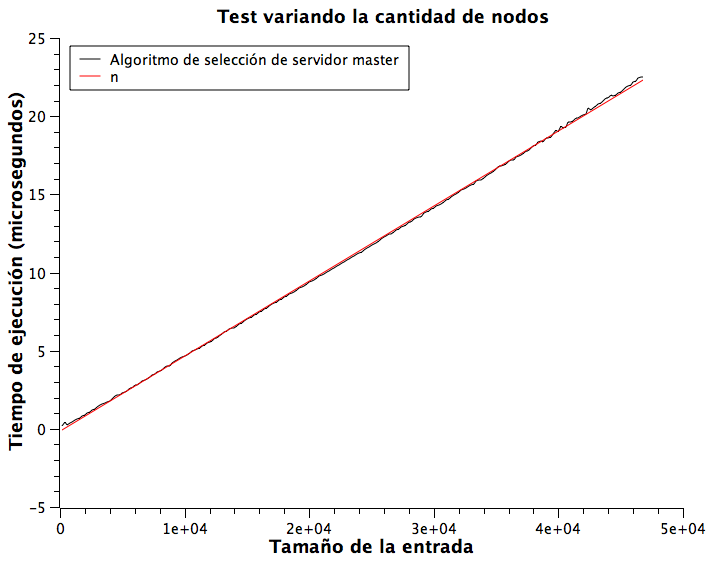
\includegraphics[width=350pt]{../tests/ej2/EJ2-nodo-var.png}
%\end{center}
\end{figure}

En este caso se puede apreciar como la comlpejidad se adapta perfectamente a los valores de entrada.\\
La función utilizada para aproximar nuestros valores resultantes luego de las distintas ejecuciones fue $A*x+B$.
En este caso, los valores que aproximan la función a nuestros datos son:

$$desde\ x = 200\ a\ x = 46.800$$
$$A  = 0,000480693152246956$$
$$B  = -0,176228394042768$$


\subsection{Preguntas adicionales}

\subsubsection{Pregunta 1}
En primer lugar, mostremos un contraejemplo en el que se pueda ver que es posible resolver las dos partes por separado de manera óptima pero que aún así haya una solución en la que la replicación termine en menos tiempo.\newline
\newline
Supongamos que tenemos el siguiente grafo:\newline

\textbf{Formato de entrada:}
$$5\ 5$$
$$4\ \ 3\ \ 1$$
$$5\ \ 3\ \ 1$$
$$3\ \ 2\ \ 1$$
$$1\ \ 5\ \ 1$$
$$3\ \ 1\ \ 1$$

\begin{figure}[H] %[h] Aqui [b] para button [t] para top
\begin{center}
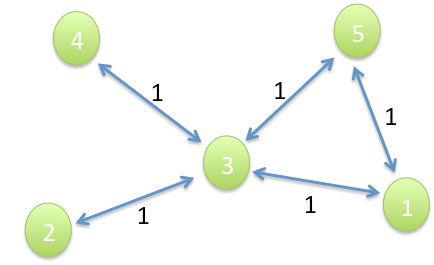
\includegraphics[width=250pt]{../imgs/pregAdicional01.jpg}
\caption{Pregunta 1 - entrada.}
\end{center}
\end{figure}
\newline
Ahora ejecutemos nuestro programa y veamos qué es lo que nos devuelve. \newline


\textbf{Formato de salida:}
$$4\ 5\ 4\ 4\ 3\ 5\ 3\ 3\ 2\ 1\ 5$$

\begin{figure}[H] %[h] Aqui [b] para button [t] para top
\begin{center}
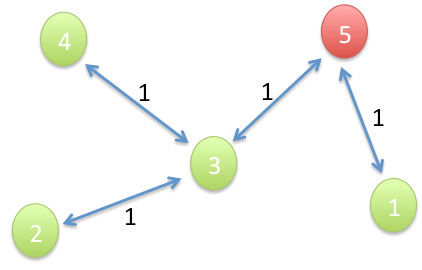
\includegraphics[width=250pt]{../imgs/pregAdicional02.jpg}
\caption{Pregunta 1 - salida.}
\end{center}
\end{figure}

\newline
Como podemos observar en el gráfico anterior, el nodo $máster$ es el 5 y el costo de replicación es igual a 2. Otra solución posible hubiera sido la que tiene al 3 como nodo $máster$ ya que ésta también tiene costo de replicación 2. \newline
\newline
Analicemos por qué nuestro algoritmo devolvió dicha solución. En primer lugar, el árbol generador mínimo ($AGM$) retornado, se encuentra conformado por las primeras cuatro aristas que ingresamos como parámetro de entrada. Ésto se debe a que nuestro algoritmo ordena primero las aristas por su peso y luego toma las menores para generar el $AGM$. En este caso, como todas las aristas tienen el mismo peso, el algoritmo no cambia su orden y genera el $AGM$ con las primeras cuatro. \newline
\newline
Ahora veamos qué ocurre si cambiamos el orden de las aristas:

\textbf{Formato de entrada:}
$$5\ 5$$
$$4\ \ 3\ \ 1$$
$$5\ \ 3\ \ 1$$
$$3\ \ 2\ \ 1$$
$$3\ \ 1\ \ 1$$
$$1\ \ 5\ \ 1$$

\newline
Para ello, cambiemos de lugar las cuarta y quinta aristas: \newline

\textbf{Formato de salida:}
$$4\ 3\ 4\ 4\ 3\ 5\ 3\ 3\ 2\ 3\ 1$$

\begin{figure}[H] %[h] Aqui [b] para button [t] para top
\begin{center}
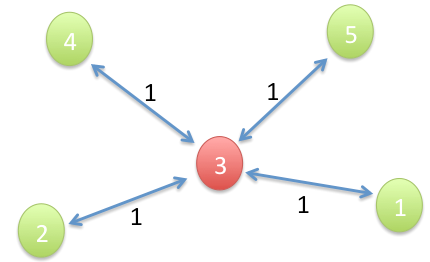
\includegraphics[width=250pt]{../imgs/pregAdicional03.jpg}
\caption{Pregunta 1 - salida2.}
\end{center}
\end{figure}

\newline
Al realizar dicho cambio, el $AGM$ resultante varía. Esto se debe a que, nuevamente, nuestro algoritmo lo genera con las primeras 4 aristas. Sin embargo, esta distribución sigue siendo solución de nuestro problema ya que el costo de sus aristas sigue siendo 4. \newline
Ahora, observemos qué sucede con nuestro nodo $máster$. El nodo máster que nos da esta solución es 3, que también era una posible solución del $AGM$ anterior. La única diferencia con la solución anterior es que, ahora, nuestro costo de replicación es igual a 1, lo que significa que éste es menor. \newline
\newline
Este es un claro ejemplo de un grafo que se resolvió dos veces de manera óptima pero cuya solución inicial indició de distinto modo en la solución del segundo ítem, donde la diferencia culminó en el orden de ingreso de los parámetros.
\newline
\newline
En términos generales, esto puede ocurrir para cualquier grafo en el que la solución del $ítem\ a$ (aplicar el algoritmo de Kruskal) no sea única. Esto se debe a que de todas las soluciones óptimás para el $ítem\ a$ y para cada una de estas, se va a encontrar la solución optima para el $ítem\ b$. Al hacer esto, vamos a encontrar un subconjunto de las soluciones posibles del  $ítem\ a$ que van a tener un menor costo de replicación que las demás.
\newline
\newline
Dos posibles soluciones a esto serian:
\begin{itemize}
\item Para todas las soluciones posibles del  $ítem\ a$, calcular el $ítem\ b$ y me quedo con la que me de menor costo de replicación.
\item Modificar el  $ítem\ a$ para que ordene primero por peso de la arista y luego por la cantidad (de mayor a menor) de nodos adyacentes que tienen ambos extremos de esta. 
\end{itemize}

\subsubsection{Pregunta 2}

 Por otro lado, veamos de qué modo puede modificarse la solución si en lugar de transmitir por $broadcast$ se lo hace por $multicast$, enviando un paquete a cada destino sin hacer copias. \newline

 La principal diferencia entre uno y otro radica en que el primero ($broadcast$) con mandar una vez la informacion le alcanza, ya que cada servidor se guarda y enviá una copia, mientras que el segundo lo que hace es enviar una copia a cada nodo, por lo que realizar un envío de un nodo $a$ a un nodo $b$ cuesta la sumatoria del costo de cada arista del camino. \newline

 Dicho lo anterior, una posible solución priorizando el costo de envió de datos es: \newline

\begin{algorithm}[H]
	\SetAlgoLined
	\caption{Minimización de Caminos entre Fábricas y Clientes}
	\KwIn{Grafo $G$}
	\KwOut{Grafo}
	\ \ \textbf{Grafo} Gmin \\
	\ \ \textbf{Entero} pesoMin = 0 \\
	\ \ \textbf{Mientras}(n \in Nodos(G)) \\
				\ \ \ \ \textbf{Grafo} G' = $Dijktra$(n,G) \\
				\ \ \ \ \textbf{Si} (pesoMin $\leq$ pesoTotal(G')) \\
	      \ \ \ \ \ \ \ Gmin = G' \\
				\ \ \ \ \textbf{FinSI} \\
		\ \ \textbf{FinMientras} \\
		\ \ \textbf{return} Gmin 
\end{algorithm}

Donde $pesoTotal$ calcula la sumatoria del peso de todas las aristas y  $Dijktra$\footnote{Cormen, Thomas H., Charles E. Leiserson, and Ronald L. Rivest. p.658} calcula los caminos mínimos de un nodo hasta todos los demás. De esta manera nos vamos quedando con aquella solución que la sumatoria de todas las aristas posea menor peso. \newline

Esta solución tiene una complejidad de $\mathcal{O}(n^{3})$ siendo n la cantidad de servidores (nodos), ya que por cada vértice aplica dicho algoritmo.\newline
